\chapter{System characterization}

\section{Verification of axial resolution}

In Section \ref{sec:axial_res}, predicitions were made about the axial resolution achievable by the FO-DOCM system. Here, these predictions are validated and limitations are explained.

\subsection{Results without AOMs}

To prevent possibly confounding factors, the system was first tested with the AOMs in place. In this case, it functions as convential time-domain OCT, with a carrier frequency determined solely by the speed of the $z$-axis scan.

The ``sample'' is replaced by a mirror for maximum possible SNR.

In this case, the $z$-axis stage was moved in increments of 100 nanometers and the DC voltage from the photodetector was acquired and stored for reach position. This ensures that the distance measured is accurate.

\begin{figure}[h!]
\centering
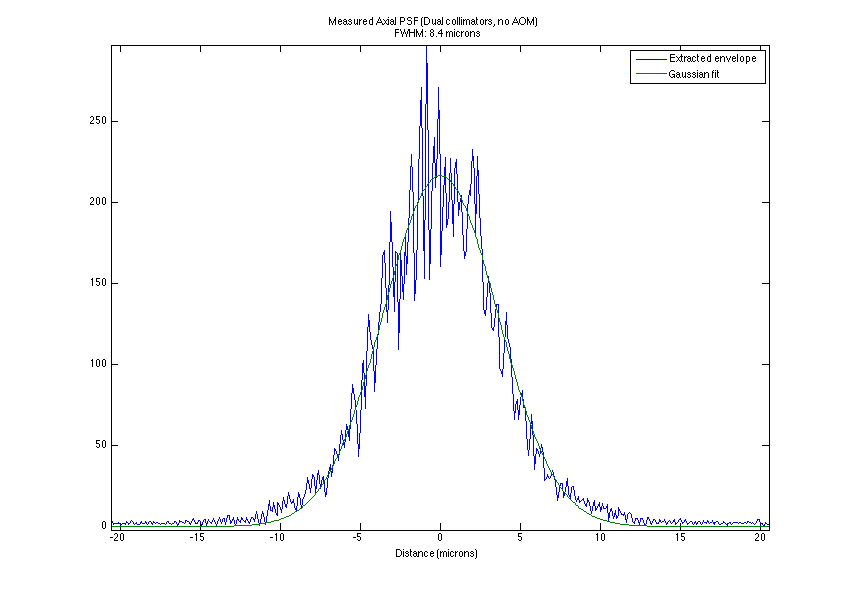
\includegraphics[width=1.0\textwidth]{Images/Results/psf-noaom.png}
\caption{The point spread function, as measured, and the best Gaussian fit.}
\end{figure}

With this method, a full width half maximum PSF width of 8.4 microns was measured. The calculated PSF is noisy as a result of the envelope detection method -- since the carrier frequency without AOMs is so much closer to the bandwidth of the PSF, the analytic signal extraction is much less exact. Furthermore, the variability in the stage position (on the order of 100nm) results in phase noise in the carrier wave that makes envelope extraction more difficult.

\subsection{Results with AOMs}

After the verification of the axial resolution without the AOMs, verification with them in place could proceed.

In a similar way, this data was acquired by moving the stage a small amount. However, DC voltage data cannot be acquired, as the relevant factor now is the amplitude of the 500 KHz carrier wave. Therefore, a small 0.1 second sample of the carrier wave was recorded for each position.

\section{Verification of transverse resolution}

To verify transverse resolution, two methods were used: a standard USAF resolution test target, and imaging polystyrene beads on a glass slide.

\section{Verification of motion resolution}

To verify motion resolution, a piezo-electric crystal was analyzed over ar range of vibrational amplitudes. These results were cross-referenced with results from the Hong et. al. OCT systems to ensure accurate measurements.

\section{Resolution of motion differentiation}

The final system verification characteristic is what we refer to as ``motion diffferentiation resolution'' -- the ability of the system to resolve the difference in vibrational amplitude between closely spaced objects.